\documentclass{beamer}
\usepackage{adjustbox}
\usepackage{textcomp}
\usepackage{booktabs}
\usepackage{amsmath}
\usepackage{xkeyval}
\usepackage{subfig}
\usepackage{todonotes}
\presetkeys{todonotes}{inline}{}
\setbeamertemplate{caption}[numbered]

\mode<presentation>{
\usetheme{Antibes}
\usecolortheme{beaver}
}

\title{Example Models in Stan}
\author{Martin Ingram}
\begin{document}
\begin{frame}
\titlepage
\end{frame}

\begin{frame}
\frametitle{What is Stan?}
\begin{columns}
\begin{column}{0.75\textwidth}
\begin{itemize}
	\item Stan is a ``probabilistic programming language''. Most importantly, it helps us do Bayesian inference.
	\item We specify our model:
	\begin{equation}
		p(\theta, y) = p(\theta) \times p(y | \theta)
	\end{equation}
	\item where $p(\theta)$ is our prior on the model parameters $\theta$ and $p(y | \theta)$ is the likelihood of the data $y$ given those parameters.
	\item Stan will give us samples of
	\begin{equation}
		p(\theta | y) = \frac{p(\theta) \times p(y | \theta)}{p(y)}
	\end{equation}
\end{itemize}
\end{column}
\begin{column}{0.25\textwidth}

\includegraphics[width=\textwidth]{stan_logo}
\end{column}
\end{columns}
\end{frame}

\begin{frame}
\frametitle{A very simple example: linear regression}
\begin{columns}
\begin{column}{0.5\textwidth}
	Model: Line with slope $a$, intercept $b$, and noise $\sigma$.

	\textbf{Prior $p(\theta)$}:
	\begin{align*}
		p(a, b, \sigma) & = p(a)p(b)p(\sigma) \\
		a, b & \sim \textrm{Uniform}(-\infty, +\infty) \\
		\sigma & \sim \textrm{Uniform}(0, +\infty)
	\end{align*}
	\textbf{Likelihood $p(y | \theta)$}:
	\begin{align*}
		y | a, b, \sigma \sim \textrm{Normal}(ax + b, \sigma^2)	
	\end{align*}
\end{column}
\begin{column}{0.5\textwidth}	
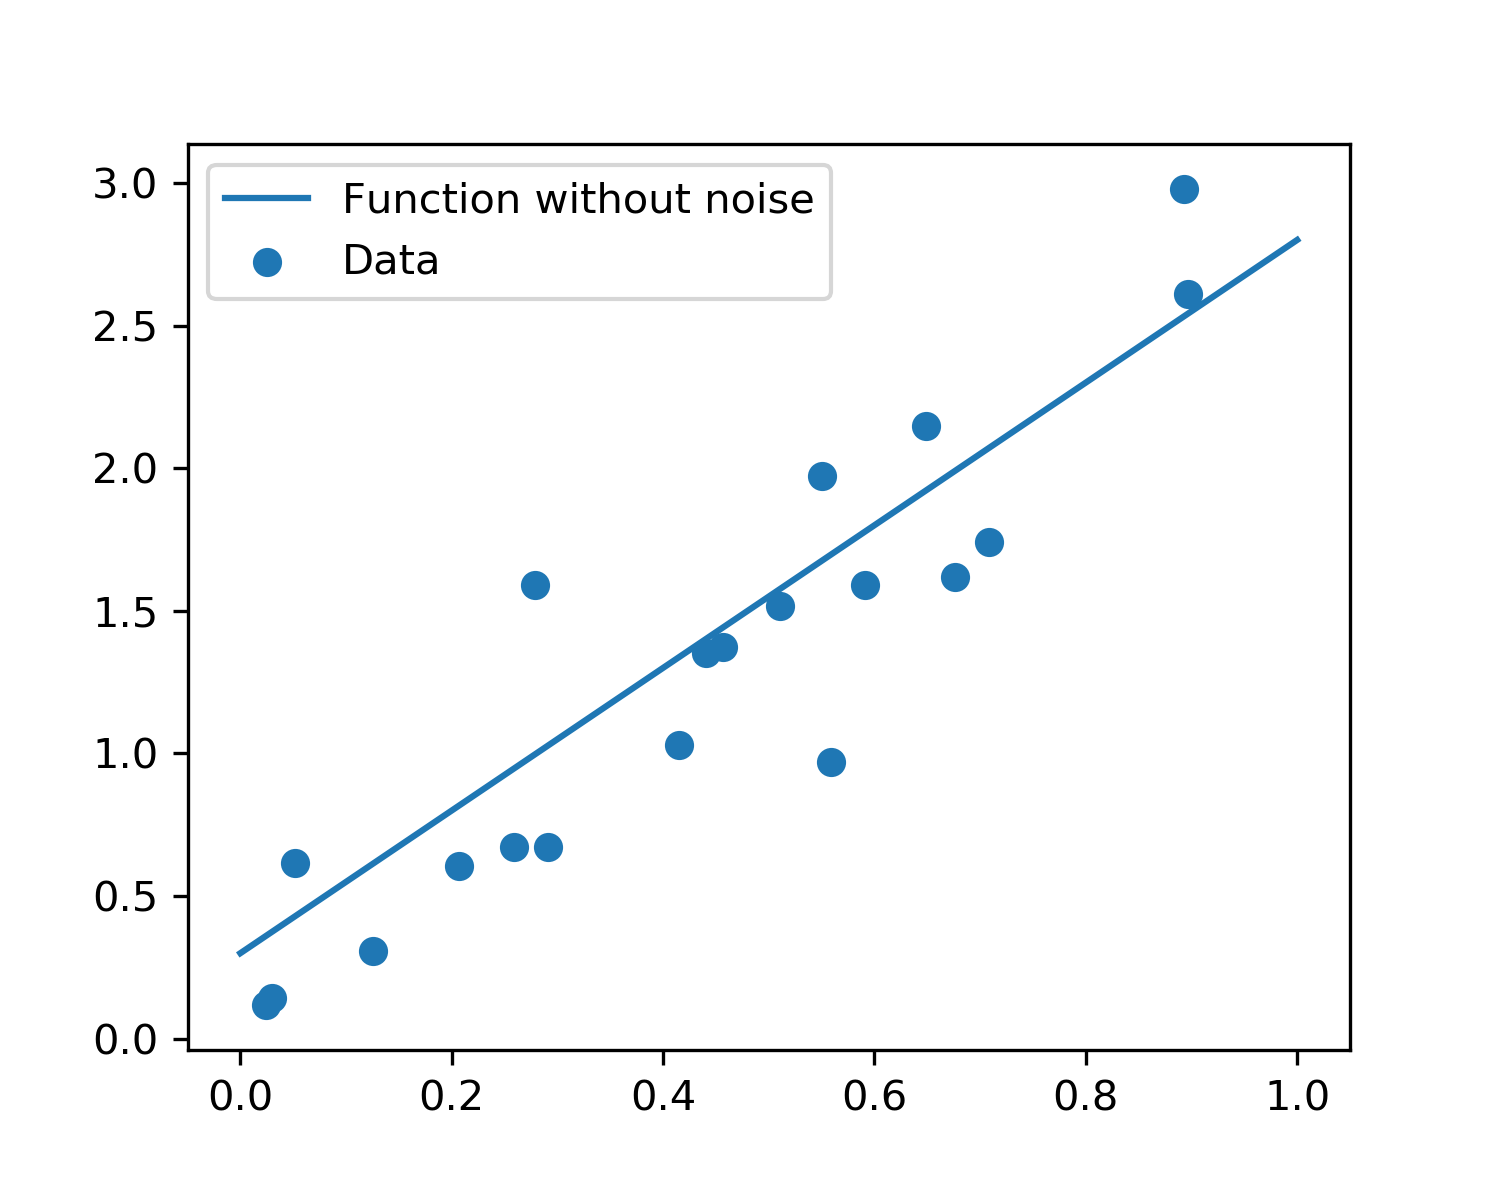
\includegraphics[width=\textwidth]{lin_reg_data}	
\end{column}
\end{columns}
\end{frame}

\begin{frame}[fragile]
\frametitle{Linear regression in Stan}
\begin{verbatim}
data {
    int N; // number of data points
    vector[N] x; // Input
    vector[N] y; // Output
}
parameters {
    real a; // Slope
    real b; // Intercept
    real<lower=0> stdev; // Standard deviation of noise
}
model {
    y ~ normal(a * x + b, stdev);
}
\end{verbatim}
\end{frame}

\begin{frame}
	\frametitle{Demo}
	Things to note:
	\begin{itemize}
		\item The $\hat{R}$ value gives us an indication of whether the model converged
		\item We can compute 95\% credible intervals easily from the posterior samples
		\item We get samples from the true posterior, not an approximation
		\item We don't really need Stan for this -- this is one of the few examples where we can compute $p(\theta | y)$ analytically
		\item Stan automatically puts flat priors (that is, uniform mass on the domain) on variables if none are specified.
	\end{itemize}
\end{frame}

\begin{frame}
	\frametitle{Hierarchical models -- 8 Schools}
	The ``Hello World'' of Stan!
\centering
\begin{figure}
\begin{tabular}{lrr}
\toprule
{} &   y &  $\sigma$ \\
\midrule
School 1 &  28 &     15 \\
School 2 &   8 &     10 \\
School 3 &  -3 &     16 \\
School 4 &   7 &     11 \\
School 5 &  -1 &      9 \\
School 6 &   1 &     11 \\
School 7 &  18 &     10 \\
School 8 &  12 &     18 \\
\bottomrule
\end{tabular}
\caption{Treatment effects from 8 schools. The schools have all received a coaching program designed to improve their SAT scores. We want to know how effective the coaching program is.}
\end{figure}
\end{frame}

\begin{frame}
	\frametitle{How do we do it?}
	\begin{itemize}
		\item ``Complete Pooling'': \emph{Single} treatment effect for all schools:
		\begin{align*}
			y_i | \theta \sim N(\theta, \sigma_i^2)	
		\end{align*}
		\item ``No pooling'': \emph{Separate} treatment effect for each school. Assume: treatment effects have nothing in common.
		\item Hierarchical models give us a third option: ``partial pooling''. Assume: treatment effects different, but drawn from the same distribution:
		\begin{align*}
			\mu & \sim \textrm{Uniform}(-\infty, +\infty) \\
			\tau & \sim \textrm{Uniform}(0, +\infty) \\
			\theta_i | \mu, \tau & \sim N(\mu, \tau^2) \\
			y_i | \theta_i & \sim N(\theta_i, \sigma_i^2)
		\end{align*}
	\end{itemize}
\end{frame}

\begin{frame}
	\frametitle{Illustration of partial pooling}
	\begin{figure}
		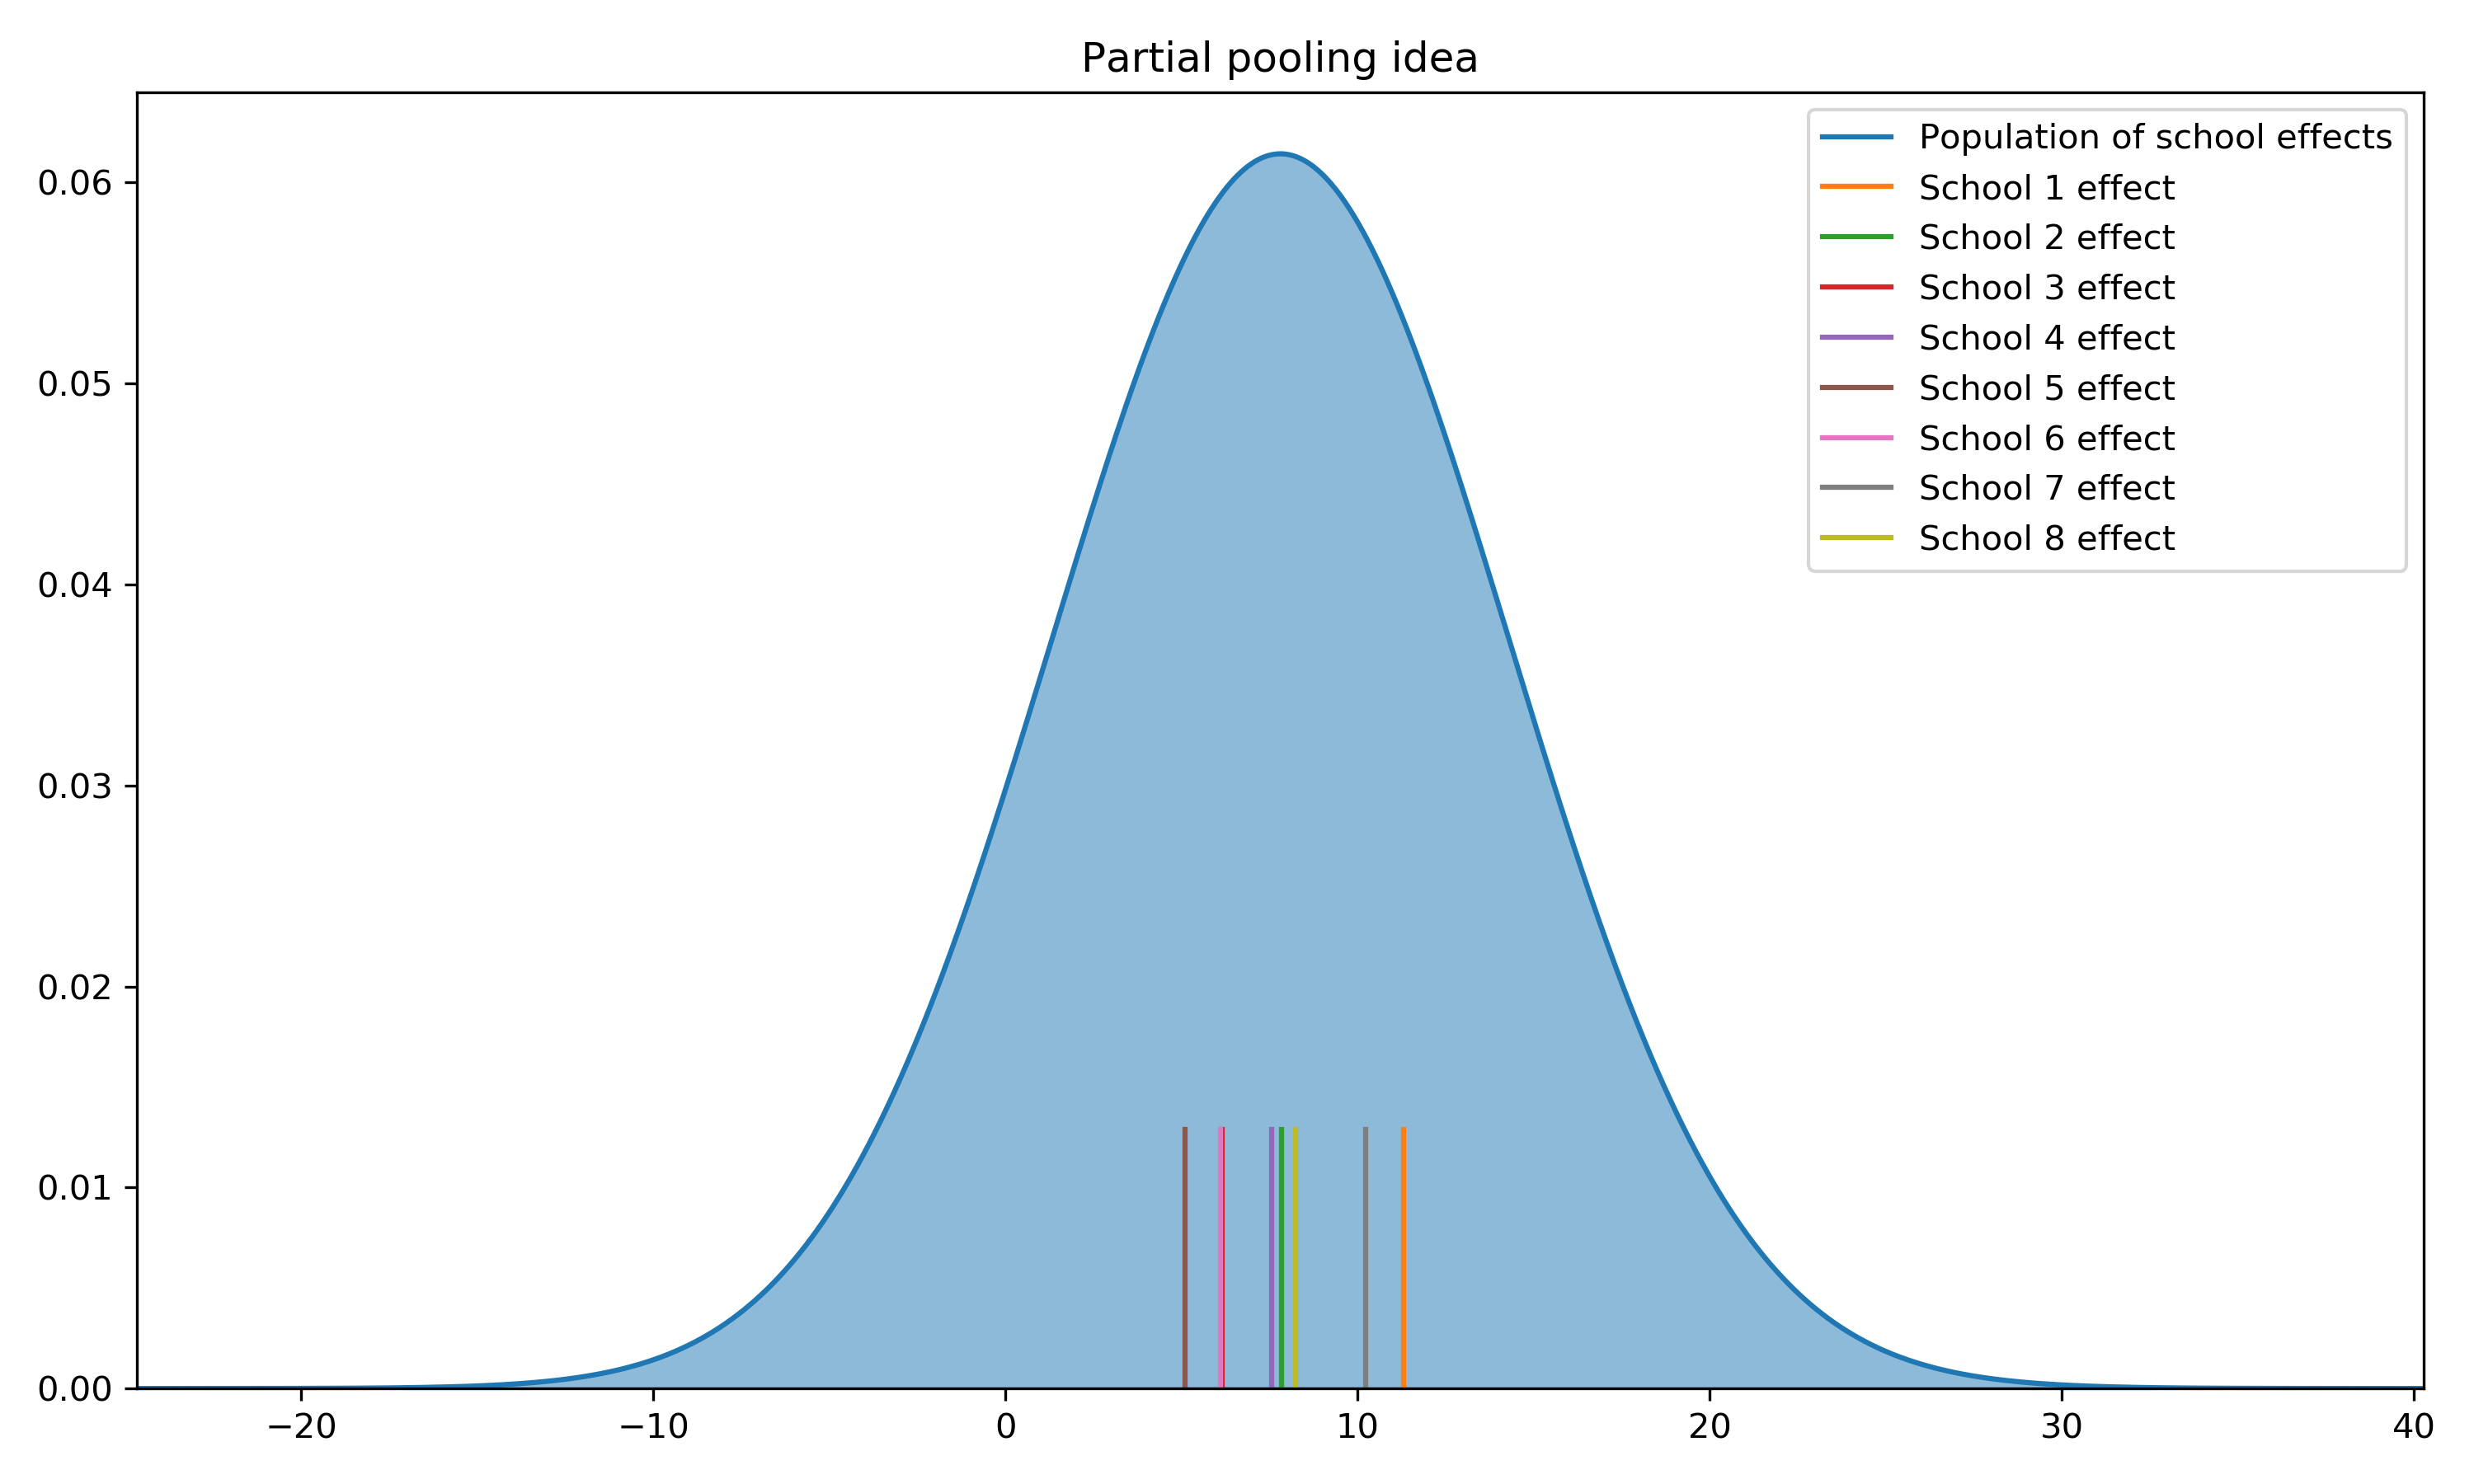
\includegraphics[width=0.8\textwidth]{partial_pooling}
		\caption{The idea behind partial pooling. We allow the school effects to be different, but we assume that they are all drawn from some population distribution, shown in blue.}		
	\end{figure}
\end{frame}

\begin{frame}[fragile]
\frametitle{Eight Schools demo in Stan}
Things to point out:
\begin{itemize}
	\item The mean treatment effect ends up looking similar, but we now allow for variation across schools.
	\item Each school gets a revised treatment estimate by ``borrowing strength'' from the other estimates.
\end{itemize}
\end{frame}

\begin{frame}
	\frametitle{AFL example}
	\begin{itemize}
		\item What if we wanted to find out AFL home advantage, accounting for team strength?
		\item Like with eight schools, we have three options:
		\begin{itemize}
			\item Complete pooling: one home advantage across all teams. But some teams do much better at home...!
			\item No pooling: A separate home advantage for all teams. But we expect that home advantages should be roughly similar across teams.
			\item Partial pooling: We draw the home advantages from a common distribution.
		\end{itemize}
	\end{itemize}
\end{frame}

\begin{frame}
\frametitle{Data \& Model}
\begin{itemize}
	\item We'll use AFL data from 2014 onwards.
	\item We give each team $i$ a separate skill $\theta$ each year $k$ (no pooling):
	\begin{align*}
		\theta_{ki} \sim N(0, 1)
	\end{align*}
	\item We give each team $i$ a separate home advantage $\gamma$ (assumed constant across seasons; flat priors on $\mu$ and $\sigma$):
	\begin{align*}
		\gamma_i | \mu_h, \sigma_h \sim N(\mu_h, \sigma_h^2)
	\end{align*}
	\item The likelihood for team $i$ to beat team $j$ at home in year $k$ is:
	\begin{align*}
		\textrm{i beats j in year k}|\theta, \gamma \sim \textrm{Bernoulli}(\textrm{logit}^{-1}(\theta_{ki} - \theta_{kj} + \gamma_i))
	\end{align*}
\end{itemize}
\end{frame}

\begin{frame}
	\frametitle{Complications}
	\begin{itemize}
		\item Sometimes the venue is home for both teams. In that case, assume no home advantage.
		\item The Bernoulli likelihood needs win or loss, so we discard draws.
	\end{itemize}
\end{frame}

\begin{frame}
\frametitle{Mean and standard deviation of home advantage in AFL since 2014}
\begin{figure}
	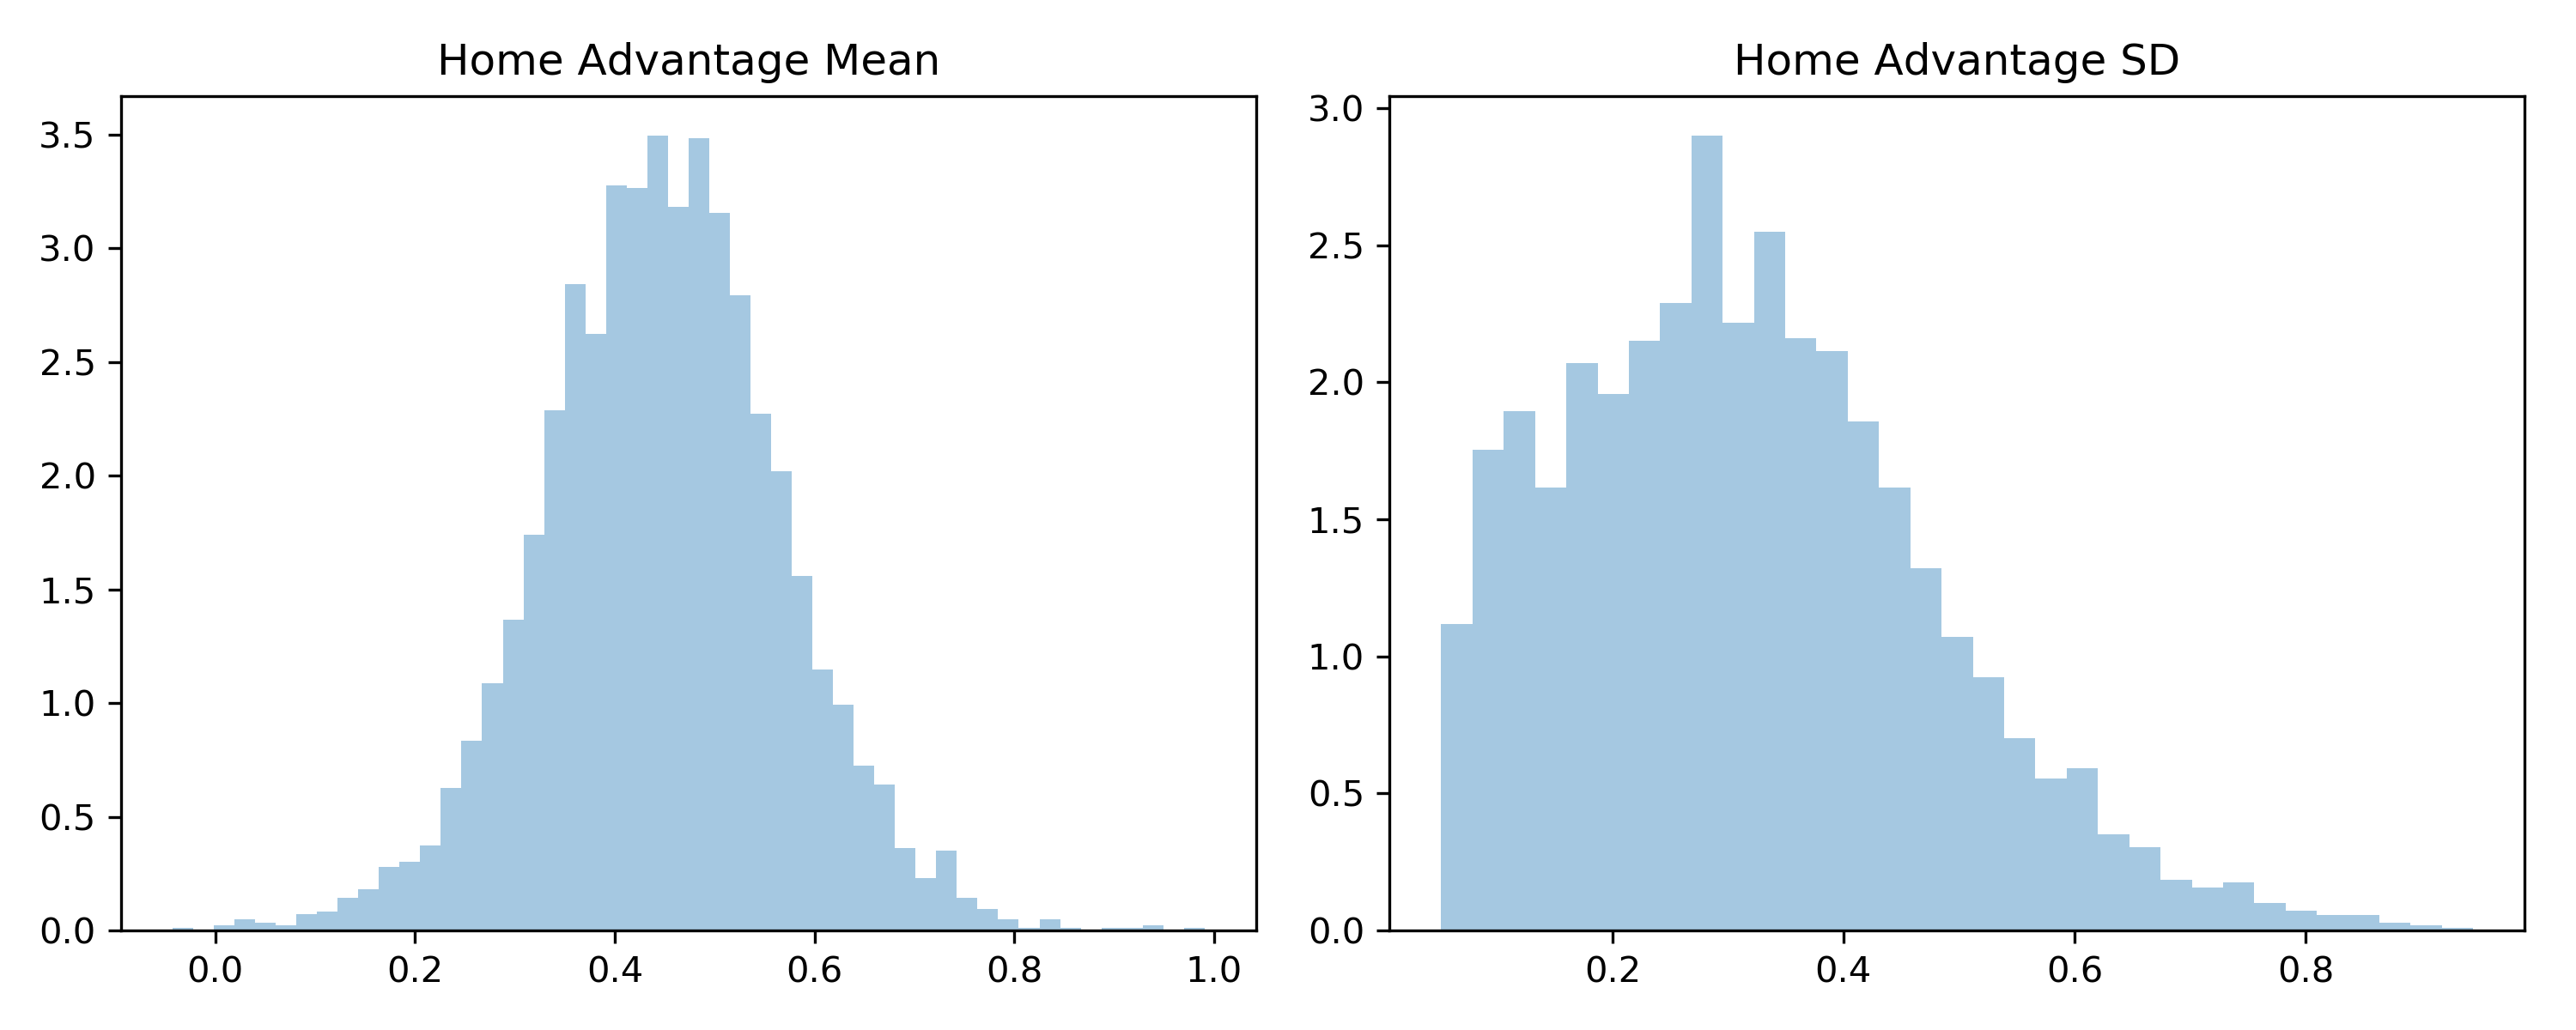
\includegraphics[width=\textwidth]{mean_var_home_ad}	
	\caption{Mean and standard deviation of home advantage in the AFL. The means of these posteriors suggest the distribution is about $0.4 \pm 0.3$. For equal teams, $0.4$ translates to +10\% win probability.}
\end{figure}
\end{frame}

\begin{frame}
	\frametitle{Home advantage estimates by team}
	\begin{figure}
	\centering
	\tiny
	\begin{tabular}{lrrrrr}
\toprule
{} &  2.5\% &   25\% &  median &   75\% &  97.5\% \\
\midrule
Geelong          &  0.22 &  0.50 &    0.69 &  0.94 &   1.51 \\
GWS Giants       &  0.13 &  0.42 &    0.57 &  0.76 &   1.19 \\
West Coast       &  0.13 &  0.41 &    0.57 &  0.76 &   1.23 \\
Adelaide         &  0.08 &  0.40 &    0.54 &  0.72 &   1.18 \\
North Melbourne  &  0.07 &  0.38 &    0.53 &  0.72 &   1.16 \\
Fremantle        &  0.07 &  0.39 &    0.53 &  0.70 &   1.11 \\
Hawthorn         &  0.02 &  0.36 &    0.52 &  0.71 &   1.14 \\
Port Adelaide    & -0.00 &  0.33 &    0.48 &  0.64 &   1.03 \\
Carlton          & -0.09 &  0.31 &    0.46 &  0.63 &   1.03 \\
Collingwood      & -0.08 &  0.30 &    0.45 &  0.62 &   1.02 \\
Essendon         & -0.11 &  0.29 &    0.45 &  0.61 &   1.03 \\
St Kilda         & -0.17 &  0.24 &    0.41 &  0.57 &   0.92 \\
Richmond         & -0.19 &  0.23 &    0.39 &  0.54 &   0.92 \\
Western Bulldogs & -0.21 &  0.22 &    0.39 &  0.55 &   0.89 \\
Gold Coast       & -0.17 &  0.23 &    0.39 &  0.54 &   0.89 \\
Sydney           & -0.39 &  0.06 &    0.26 &  0.41 &   0.67 \\
Melbourne        & -0.57 & -0.03 &    0.21 &  0.40 &   0.67 \\
Brisbane         & -0.60 & -0.09 &    0.18 &  0.37 &   0.62 \\
\bottomrule
\end{tabular}
\caption{Home advantage estimates $\gamma$ for all AFL teams.}
\end{figure}
\end{frame}

\begin{frame}
	\frametitle{Best teams this year}
	\begin{figure}
	\tiny
	\begin{tabular}{lrrrrr}
\toprule
{} &  2.5\% &   25\% &  median &   75\% &  97.5\% \\
\midrule
Richmond         &  0.34 &  1.01 &    1.34 &  1.69 &   2.35 \\
Sydney           & -0.12 &  0.49 &    0.83 &  1.19 &   1.84 \\
West Coast       & -0.07 &  0.52 &    0.82 &  1.15 &   1.80 \\
Hawthorn         & -0.31 &  0.26 &    0.60 &  0.94 &   1.62 \\
Collingwood      & -0.38 &  0.25 &    0.56 &  0.88 &   1.52 \\
GWS Giants       & -0.46 &  0.17 &    0.53 &  0.90 &   1.56 \\
Melbourne        & -0.49 &  0.14 &    0.48 &  0.80 &   1.41 \\
Geelong          & -0.64 & -0.03 &    0.31 &  0.65 &   1.30 \\
Port Adelaide    & -0.74 & -0.06 &    0.27 &  0.61 &   1.24 \\
Essendon         & -0.79 & -0.15 &    0.19 &  0.51 &   1.14 \\
Adelaide         & -0.87 & -0.20 &    0.14 &  0.46 &   1.04 \\
North Melbourne  & -0.98 & -0.33 &    0.01 &  0.33 &   0.95 \\
Western Bulldogs & -1.43 & -0.81 &   -0.47 & -0.17 &   0.42 \\
Fremantle        & -1.48 & -0.83 &   -0.49 & -0.15 &   0.46 \\
Brisbane         & -1.99 & -1.26 &   -0.91 & -0.56 &   0.07 \\
St Kilda         & -2.12 & -1.41 &   -1.03 & -0.67 &  -0.06 \\
Gold Coast       & -2.47 & -1.74 &   -1.34 & -0.98 &  -0.34 \\
Carlton          & -2.89 & -2.16 &   -1.79 & -1.45 &  -0.79 \\
\bottomrule
\end{tabular}	
\caption{Team skills $\theta$ for this season.}
\end{figure}
\end{frame}

\begin{frame}
\frametitle{Conclusions}
\begin{itemize}
	\item Stan is extremely flexible. If you can write down the model, Stan can (probably) sample it.
	\item Hierarchical models are often useful. They allow you to ``borrow strength'' between estimates.
	\item Quick plug: Stan is not the only probabilistic programming language. In particular, in R, Nick is working on a framework called greta which uses tensorflow to do sampling more quickly
\end{itemize}
\end{frame}

\end{document}
